\section*{Learning Objectives}

\begin{itemize}
\item Master the Gram-Schmidt algorithm
\item Explore some of its uses
\item Regression
\item Debugging, or finding and fixing errors in your code
\end{itemize}

\section*{Outcomes} 
\begin{itemize}
\item In a set of orthogonal vectors, each vector forms a right angle with respect to the other vectors in the set
\item If a vector is non-zero, we can easily normalize its length to one
\item In a set of orthonormal vectors, each vector has length one and forms a right angle with respect to the other vectors in the set 
\item Gram-Schmidt applied to a set of linearly independent vectors produces a set of orthogonal vectors, and with one small modification, we can produce a set of orthonormal vectors
\item Gram-Schmidt provides an easy way to compute the null space of a matrix
\end{itemize}

\vspace*{1cm}

\textbf{Either download Lab7 from our Canvas site or open up a Jupyter notebook so that you can enter code as we go. It is suggested that you have line numbering toggled on.}  

\newpage

This lab goes all in on the Gram-Schmidt Process. When you are done with the lab, you should feel that you ``own'' the algorithm. \\

Julia has a command for computing the inner product, aka dot product, of two vectors. Surprise, the command is called \texttt{dot}. We'll show you how to use it.

\begin{lstlisting}[language=Julia,style=mystyle]
# The dot comamnd is part of the LinearAlgebra package.
#
using LinearAlgebra
#
u = [1, 2, 3, 4, 5]
v = [6, 7, 8, 9, 10]

uDOTv = dot(u,v)
\end{lstlisting}
\textbf{Output} 
\begin{verbatim}
130
\end{verbatim}
You can easily compute the dot product without the LinearAlgebra Package. 

\begin{lstlisting}[language=Julia,style=mystyle]
# The dot command computes u'*v; here is the proof!
u'*v 
\end{lstlisting}
\textbf{Output} 
\begin{verbatim}
130
\end{verbatim}

Normalizing the length of vectors to one is a pain by hand. But in Julia, it's such a snap that we will soon incorporate it directly into the Gram-Schmidt process. 

\begin{lstlisting}[language=Julia,style=mystyle]
# The norm command is part of the LinearAlgebra Package, which we already ran
@show norm(v)
w = v /norm(v)
@show norm(w)
w 
\end{lstlisting}
\textbf{Output} 
\begin{verbatim}
norm(v) = 18.16590212458495
norm(w) = 1.0

5-element Vector{Float64}:
 0.3302891295379082
 0.3853373177942262
 0.4403855060505443
 0.4954336943068623
 0.5504818825631803
\end{verbatim}

\section{Orthogonal Vectors}

Suppose that $\{ u_1, u_2\}$ is a set of linearly independent vectors. The Gram-Schmidt Process builds from them an orthogonal set of vectors that spans the same set of vectors as $\{ u_1, u_2\}$. It works as follows:\\

\textbf{Step 1:} $v_1 := u_1$ \\

\textbf{Step 2:} $v_2 := u_2  - a_2 v_1$, where we seek to choose $a_2$ such that $v_2 \bullet v_1 = 0$. We compute
\begin{align*}
    v_2 \bullet v_1 &  = \left( u_2  - a_2 v_1 \right) \bullet  v_1 \\
    &= u_2 \bullet v_1 - a_2 v_1 \bullet v_1.
\end{align*}
If $ v_1 \bullet v_1\neq 0$, then we can set $u_2 \bullet v_1 - a_2 v_1 \bullet v_1 = 0$ and solve for $a_2$, namely
$$a_2 = \frac{u_2 \bullet v_1}{v_1 \bullet v_1}. $$
\\

\begin{tcolorbox}
\textbf{Important Formula to Build $\boldsymbol{v_1 \perp v_2}$ from $\boldsymbol{u_1}$ and $\boldsymbol{u_2}$ while Preserving Spans}
\begin{equation}
    \label{eq:OrthognalProjection01}
    \begin{aligned}
    v_1 &= u_1\\
    v_2 &= u_2 -  \left(\frac{u_2 \bullet v_1}{v_1 \bullet v_1}\right) v_1\\
    \\ 
    \spanof{v_1}&=\spanof{u_1}\\
    \spanof{v_1, v_2}&= \spanof{u_1, u_2}
     \end{aligned}
\end{equation}
\end{tcolorbox}

We illustrate the above step by step.

\begin{lstlisting}[language=Julia,style=mystyle]
using Random
Random.seed!(2022)
u1 = rand(4,1)
u2 = rand(4,1)
U = [u1 u2]
@show det(U'*U) # non-zero means u1 and u2 are independent
# G-S on two vectors (see grey box above)
@show v1 = u1
@show v2 = u2 - ( dot(u2,v1)/dot(v1,v1) )*v1
V = [v1 v2]
@show dot(v1,v2) # should be zero
println(" ") # Will print a space
@show det(V'*V) # non-zero means v1 and v2 are independent
V
\end{lstlisting}
\textbf{Output} 
\begin{verbatim}
det(U' * U) = 0.32941782975491707
v1 = u1 = [0.7982589547203172; 0.8998485508054206; 0.15010598805721265;
0.1749482291443072]
v2 = u2 - (dot(u2, v1) / dot(v1, v1)) * v1 = [-0.04289157616244632; -0.07773177980842272;
0.3598021757771466; 0.28681029417179305]
dot(v1, v2) = -1.2642012348321895e-17
 
det(V' * V) = 0.32941782975491707

4×2 Matrix{Float64}:
 0.798259  -0.0428916
 0.899849  -0.0777318
 0.150106   0.359802
 0.174948   0.28681
\end{verbatim}

\begin{lstlisting}[language=Julia,style=mystyle]
v1=v1/norm(v1)  
v2=v2/norm(v2)
# 
V= [v1 v2]  # now columns are orthonormal vectors
@show det(V'*V) # non-zero implies linearly independent
@show V'*V - [v1'*v1  v1'*v2; v2'*v1 v2'*v2]
V'*V
\end{lstlisting}
\textbf{Output} 
\begin{verbatim}
det(V' * V) = 1.0000000000000004
V' * V - [v1' * v1  v1' * v2; v2' * v1  v2' * v2] = [0.0 0.0; 0.0 0.0]

2×2 Matrix{Float64}:
  1.0          -1.34268e-17
 -1.34268e-17   1.0
\end{verbatim}


\begin{lstlisting}[language=Julia,style=mystyle]
# A helper function to zero out small entries of a matrix or vector
function cleanUp(A,tol=1e-10)
    B=copy(A)
    indicesSmall=findall(x->x<tol, abs.(B))
    B[indicesSmall]=0.0*abs.(B[indicesSmall])
    return B
end
\end{lstlisting}
\textbf{Output} 
\begin{verbatim}
cleanUp (generic function with 2 methods)
\end{verbatim}


\begin{lstlisting}[language=Julia,style=mystyle]
cleanUp(V'*V)
\end{lstlisting}
\textbf{Output} 
\begin{verbatim}
2×2 Matrix{Float64}:
 1.0  0.0
 0.0  1.0
\end{verbatim}

\section{The Span Condition}

Next will check that $\spanof{u_1, u_2} = \spanof{v_1, v_2}$, where we recall that computing the span of a set of vectors means determining ``all possible linear combinations'', which seems like a lot of work! However, if we show that
\begin{align}
\label{eq:u1}
    u_1 & \in \spanof{v_1, v_2}\\
\label{eq:u2}
    u_2 & \in \spanof{v_1, v_2},
\end{align}
it then follows that $\spanof{u_1, u_2} \subset \spanof{v_1, v_2}$. If we also show that
\begin{align}
\label{eq:v1}
    v_1 & \in \spanof{u_1, u_2} \\
\label{eq:v2}
    v_2 & \in \spanof{u_1, u_2}, 
\end{align}
we'll have that $\spanof{v_1, v_2} \subset \spanof{u_1, u_2}$. Moreover, for any two \textbf{subsets} $A$ and $B$, the conditions $A \subset B$ and $B \subset A$ are equivalent to $A=B$. Applying this to $\spanof{u_1, u_2}$ and $\spanof{v_1, v_2}$, yields
$$\big(\spanof{u_1, u_2} \subset \spanof{v_1, v_2}\big) \text{\bf and } \big(\spanof{v_1, v_2} \subset \spanof{u_1, u_2} \big) \iff \big(\spanof{u_1, u_2} = \spanof{v_1, v_2}\big).$$

Because $u_1 = v_1$, the conditions \eqref{eq:u1} and \eqref{eq:v1} are immediate. Hence, we only need to show conditions \eqref{eq:u2} and \eqref{eq:v2}, 
% \begin{align*}
%     u_2 & \in \spanof{v_1, v_2}\\
%     & \text{and} \\
%     v_2 & \in \spanof{u_1, u_2}, \\
% \end{align*}
that is, $u_2$ can be written as a linear combination of $v_1$ and $v_2$, and similarly, $v_2$ can be written as a linear combination of $u_1$ and $u_2$.\\

In our textbook, we show these conditions analytically. Below, we verify them in code!\\

\begin{lstlisting}[language=Julia,style=mystyle]
# We check the span conditions
# including the obvious: u1 = v1 and v1 = u1
@show u1 - v1 
println(" ")
# define
a1 = -dot(u2,v1)/dot(v1,v1)
a2 = 1
# check v2 =  a*u1 + a2*u2 
@show v2 - (a1*u1 + a2*u2)
println(" ")
# define
b1 = dot(u2,v1)/dot(v1,v1)
b2 = 1
# check u2 =  b1*v1 + b2*v2 
@show u2 - (b1*v1 + b2*v2)
\end{lstlisting}
\textbf{Output} 
\begin{verbatim}
u1 - v1 = [0.0; 0.0; 0.0; 0.0]
 
v2 - (a1 * u1 + a2 * u2) = [0.0; 0.0; 0.0; 0.0]
 
u2 - (b1 * v1 + b2 * v2) = [0.0; 0.0; 0.0; 0.0]

4×1 Matrix{Float64}:
 0.0
 0.0
 0.0
 0.0
\end{verbatim}

Here are the analytical calculations, in case you are interested,
$$ \large
 \begin{aligned}
 v_1 & = u_1 \\
 v_2 &= u_2 - \left(\frac{u_2 \bullet v_1}{v_1 \bullet v_1}\right) v_1 \\
	\end{aligned}
$$
we deduce that
$$\boxed{\bf  \large  v_2 = a_1 u_1 + a_2 u_2 } $$
with 
$$  \large
 \begin{aligned}
a_1 &= -\left(\frac{u_2 \bullet v_1}{v_1 \bullet v_1}\right)\\
a_2 &= 1
\end{aligned}
$$
and
 $$ \boxed{ \bf \large u_2 = b_1 v_1 + b_2 v_2}$$
with 
$$  \large
 \begin{aligned}
b_1 &=  \left(\frac{u_2 \bullet v_1}{v_1 \bullet v_1}\right)\\
b_2 &= 1
\end{aligned}
$$

\section{Graphical Interpretation of Orthogonal Vectors and Another way to Understand the Span Condition}

Figure~\ref{fig:OrthognalVectors} provides a graphical illustration of the action of Gram-Schmidt on a pair of linearly independent vectors $\{u_1, u_2 \}$. Figure~\ref{fig:OrthognalVectors}-(a) shows two randomly generated vectors. Then we apply \textbf{Gram-Schmidt with normalization to produce orthonormal vectors} $\{v_1, v_2 \}$, as shown in Fig.~\ref{fig:OrthognalVectors}-(b).
$$
    \begin{aligned}
    v_1 &= u_1\\
    v_1 &= v_1/||v_1|| \\
    v_2 &= u_2 -  \left(u_2 \bullet v_1 \right) v_1\\
    v_2 & = v_2/||v_2||
     \end{aligned}
$$


\begin{figure}[hbt!]%
\centering
\subfloat[]{%
    \label{fig:u1u2}%
	\centering
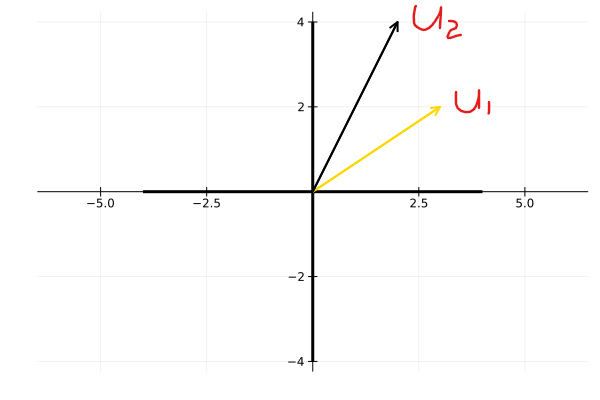
\includegraphics[width=0.45\columnwidth]{graphics/Chap07/u1u2.png}}%
\hspace{5pt}%
\subfloat[]{%
    \label{fig:v1v2}%
	\centering
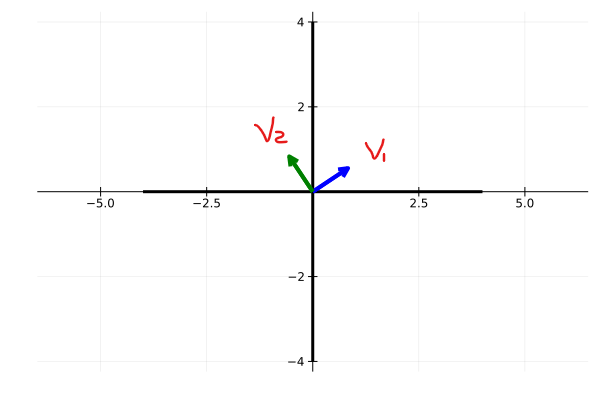
\includegraphics[width=0.45\columnwidth]{graphics/Chap07/v1v2.png}}%
\hspace{5pt}%
\subfloat[]{%
    \label{fig:u2v1v2}%
	\centering
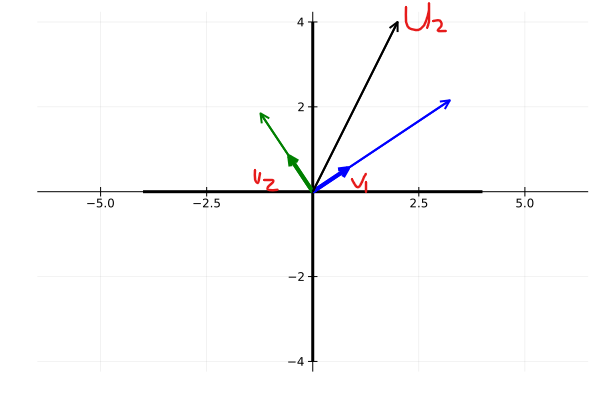
\includegraphics[width=0.45\columnwidth]{graphics/Chap07/u2v1v2.png}}%
\hspace{5pt}%
    \subfloat[]{%
    \label{fig:u2v1plusv2}%
	\centering
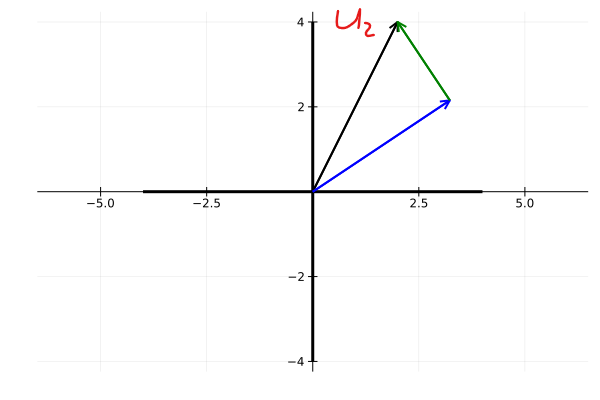
\includegraphics[width=0.45\columnwidth]{graphics/Chap07/u2v1plusv2.png}}%
    \caption[]{What does Gram-Schmidt do to a pair of linearly independent vectors? (a) $\{u_1, u_2 \}$ are linearly independent, but they do not form a right angle. (b) $\{v_1, v_2 \}$ is an \textbf{orthonormal} set produced by applying Gram-Schmidt to $\{u_1, u_2 \}$. They clearly form a right angle. (c)  The thin blue vector is $(u_2 \bullet v_1)\cdot v_1$. It goes by two names, the projection of $u_2$ along the direction $v_1$ or the component of $u_2$ along the direction $v_1$. The thin green vector is $(u_2 \bullet v_2)\cdot v_2$. It goes by two names, the projection of $u_2$ along the direction $v_2$ or the component of $u_2$ along the direction $v_2$. (d) From Gram-Schmidt, we know that $u_2 = (u_2 \bullet v_1)\cdot v_1 +(u_2 \bullet v_2)\cdot v_2 $. This last plot shows the addition of the two vectors using the head to tail notion of vector addition that you may have come across in a physics course.}
    \label{fig:OrthognalVectors}
\end{figure}

 Because $\spanof{v_1, v_2}= \spanof{u_1, u_2}$, we know that we can express $u_1$ and $u_2$ as linear combinations of $v_1$ and $v_2$. When $\{v_1, v_2 \}$ are \textbf{orthonormal}, it is very easy to compute the linear combinations
$$
\begin{aligned}
u_1 & =   \underbrace{\left(u_1 \bullet v_1 \right)}_{\alpha_1} v_1 +  \underbrace{\left(u_1 \bullet v_2 \right)}_{\alpha_2} v_2 = \alpha_1 v_1 + \alpha_2 v_2\\
\\
u_2 & =   \underbrace{\left(u_2 \bullet v_1 \right)}_{\beta_1} v_1 +  \underbrace{\left(u_2 \bullet v_2 \right)}_{\beta_2} v_2 = \beta_1 v_1 + \beta_2 v_2.
\end{aligned}
$$
Yes, it is worth repeating: when $\{v_1, v_2 \}$ are \textbf{orthonormal}, computing the coefficients in the linear combination is very easy. Figure~\ref{fig:OrthognalVectors}-(c) shows the vector $u_2$ and the two parts of its linear combination in terms of $\{v_1, v_2 \}$; namely, the thin blue vector is the component of $u_2$ along $v_1$, namely $\left(u_2 \bullet v_1 \right) v_1$, while the thin green line is the component of $u_2$ along $v_2$, namely $\left(u_2 \bullet v_2 \right) v_2$. Figure~\ref{fig:OrthognalVectors}-(d) shows that indeed, $u_2 =   \left(u_2 \bullet v_1 \right) v_1 +  \left(u_2 \bullet v_2 \right) v_2$, the sum of the two components.\\

When $\{v_1, v_2 \}$ are \textbf{orthogonal but not orthonormal}, the expressions are still quite handy,
$$
\begin{aligned}
u_1 & =   \underbrace{\left(\frac{u_1 \bullet v_1}{v_1 \bullet v_1}\right)}_{\alpha_1} v_1 +  \underbrace{\left(\frac{u_1 \bullet v_2}{v_2 \bullet v_2}\right)}_{\alpha_2} v_2 = \alpha_1 v_1 + \alpha_2 v_2\\
\\
u_2 & =   \underbrace{\left(\frac{u_2 \bullet v_1}{v_1 \bullet v_1}\right)}_{\beta_1} v_1 +  \underbrace{\left(\frac{u_2 \bullet v_2}{v_2 \bullet v_2}\right)}_{\beta_2} v_2 = \beta_1 v_1 + \beta_2 v_2.
\end{aligned}
$$

\begin{lstlisting}[language=Julia,style=mystyle]
# This code generates the plots in Figure 7.1
using Random
Random.seed!(31415926535897932384626433)
u1 = 3*randn(2,1)
u2 = 4*randn(2,1)
u1=[3; 2]
u2=[2; 4]
U = [u1 u2]
@show det(U'*U) # non-zero means independent
# G-S on two vectors (see big green box below)
@show v1 = u1
@show v2 = u2 - ( dot(u2,v1)/dot(v1,v1) )*v1

v1 = v1/norm(v1)
v2 = v2/norm(v2)

t=LinRange(-4, 4,10); t=collect(t)
zero=0.0*t;

p1=plot(t,0.0.*t, color=:black, lw=3, legend=false, aspect_ratio=:equal,framestyle = :origin)
plot!(0.0.*t,t, color=:black, lw=3, legend=false)

plot!([0;u1[1:1]],[0;u1[2:2]], arrow=true, color=:gold, lw=2 )
plot!([0;u2[1:1]],[0;u2[2:2]], arrow=true, color=:black, lw=2 )

p2=plot(t,0.0.*t, color=:black, lw=3, legend=false, aspect_ratio=:equal,framestyle = :origin)
plot!(0.0.*t,t, color=:black, lw=3, legend=false)

plot!([0;v1[1:1]],[0;v1[2:2]], arrow=true, color=:blue, lw=4 )
plot!([0;v2[1:1]],[0;v2[2:2]], arrow=true, color=:green, lw=4 )


p3=plot(t,0.0.*t, color=:black, lw=3, legend=false, aspect_ratio=:equal,framestyle = :origin)
plot!(0.0.*t,t, color=:black, lw=3, legend=false)

u2Projv1 = ( dot(u2,v1)/dot(v1,v1) )*v1
u2Projv2 = ( dot(u2,v2)/dot(v2,v2) )*v2

plot!([0;u2Projv1[1:1]],[0;u2Projv1[2:2]], arrow=true, color=:blue, lw=2 )
plot!([0;u2Projv2[1:1]],[0;u2Projv2[2:2]], arrow=true, color=:green, lw=2 )

plot!([0;v1[1:1]],[0;v1[2:2]], arrow=true, color=:blue, lw=4 )
plot!([0;v2[1:1]],[0;v2[2:2]], arrow=true, color=:green, lw=4 )
plot!([0;u2[1:1]],[0;u2[2:2]], arrow=true, color=:black, lw=2 )


p4=plot(t,0.0.*t, color=:black, lw=3, legend=false, aspect_ratio=:equal,framestyle = :origin)
plot!(0.0.*t,t, color=:black, lw=3, legend=false)

plot!([0;u2[1:1]],[0;u2[2:2]], arrow=true, color=:black, lw=2 )

plot!([0;u2Projv1[1:1]],[0;u2Projv1[2:2]], arrow=true, color=:blue, lw=2 )
plot!([0;u2Projv2[1:1]].+u2Projv1[1:1],[0;u2Projv2[2:2]].+u2Projv1[2:2], arrow=true, color=:green, lw=2 )

display(p1)
display(p2)
display(p3)
display(p4)
\end{lstlisting}
\textbf{Output} 

Plots as shown in Fig.~\ref{fig:OrthognalVectors}, though without the beautiful handwritten labels.


% \begin{lstlisting}[language=Julia,style=mystyle]

% \end{lstlisting}
% \textbf{Output} 
% \begin{verbatim}

% \end{verbatim}

% \begin{lstlisting}[language=Julia,style=mystyle]

% \end{lstlisting}
% \textbf{Output} 
% \begin{verbatim}

% \end{verbatim}

\section{Gram-Schmidt Algorithm on a Set of four Vectors}

The Gram-Schmidt Algorithm takes a set of linearly independent vectors and creates a set of orthogonal vectors that is (i) also linearly independent, and (ii), spans the same subspace as the original vectors. Here is the algorithm written out for a set of four linearly independent vectors. The hope is that you see the pattern and hence are ready to put the algorithm into a \texttt{for\, loop}.\\

\begin{tcolorbox}[sharp corners, colback=green!30, colframe=green!80!blue, title=\textbf{\Large Gram-Schmidt Process for 4 Vectors
}]
Suppose that that the set of vectors $\{ u_1, u_2, u_3, u_4\}$ is linearly independent. Then the vectors  $\{ v_1, v_2, v_3, v_4\}$ are orthogonal, where
$$
 \begin{aligned}
 v_1 & = u_1 \\
 v_2 &= u_2 - \left(\frac{u_2 \bullet v_1}{v_1 \bullet v_1}\right) v_1 \bigskip \\
 v_3 &= u_3 -\left(\frac{u_3 \bullet v_1}{v_1 \bullet v_1}\right) v_1 - \left(\frac{u_3 \bullet v_2}{v_2 \bullet v_2}\right) v_2 \\
 v_4 & = u_4  - \left(\frac{u_4 \bullet v_1}{v_1 \bullet v_1}\right) v_1 - \left(\frac{u_4 \bullet v_2}{v_2 \bullet v_2}\right) v_2 - \left(\frac{u_4 \bullet v_3}{v_3 \bullet v_3}\right) v_3
	\end{aligned}
$$


Could you write out the line for a fifth vector? 
\end{tcolorbox}

\begin{lstlisting}[language=Julia,style=mystyle]
using Random
Random.seed!(2525)
u1 = rand(4,1)
u2 = rand(4,1)
u3 = rand(4,1)
u4 = rand(4,1)
# G-S on four vectors (see big green box)
v1 = u1 # k=1
v2 = u2 - ( dot(u2,v1)/dot(v1,v1) )*v1  # k=2, i = 1:1
v3 = u3 - ( dot(u3,v1)/dot(v1,v1) )*v1 - ( dot(u3,v2)/dot(v2,v2) )*v2 # k=3, i = 1:2
v4 = u4 - ( dot(u4,v1)/dot(v1,v1) )*v1 - ( dot(u4,v2)/dot(v2,v2) )*v2 - ( dot(u4,v3)/dot(v3,v3) )*v3 # k=4, i = 1:3
\end{lstlisting}
\textbf{Output} 
\begin{verbatim}
4×4 Matrix{Float64}:
 2.54741  0.0       0.0        0.0
 0.0      0.183229  0.0        0.0
 0.0      0.0       0.0246929  0.0
 0.0      0.0       0.0        0.643923
\end{verbatim}


We define $V:=\left[ \begin{array}{cccc} v_1 & v_2 & v_3 & v_4 \end{array} \right] $ and note that 
 $$V^\top V = \left[ \begin{array}{c} v_1^\top  \\ v_2^\top \\ v_3^\top \\ v_4 \end{array} \right] \cdot \left[ \begin{array}{cccc} v_1 & v_2 & v_3 & v_4 \end{array} \right] = \left[ \begin{array}{cccc}  
 v_1^\top \cdot v_1 &  v_1^\top \cdot v_2 &  v_1^\top \cdot v_3 &  v_1^\top \cdot v_4  \\
  v_2^\top \cdot v_1 &  v_2^\top \cdot v_2 &  v_2^\top \cdot v_3 &  v_2^\top \cdot v_4  \\
   v_3^\top \cdot v_1 &  v_3^\top \cdot v_2 &  v_3^\top \cdot v_3 &  v_3^\top \cdot v_4  \\
   v_4^\top \cdot v_1 &  v_4^\top \cdot v_2 &  v_4^\top \cdot v_3 &  v_4^\top \cdot v_4
 \end{array} 
  \right],$$
  that is, 
  $$\left[V^\top V \right]_{ij} := v_i^\top \cdot v_j = v_i \bullet v_j .$$
Therefore, if the set $\{ v_1, v_2, v_3, v_4\}$ is orthogonal, we should have
 $$V^\top V = \left[ \begin{array}{c} v_1^\top  \\ v_2^\top \\ v_3^\top \\ v_4 \end{array} \right] \cdot \left[ \begin{array}{cccc} v_1 & v_2 & v_3 & v_4 \end{array} \right] = \left[ \begin{array}{cccc}  
||v_1||^2 & 0 & 0 & 0 \\
0 & ||v_2||^2 & 0 & 0 \\
0 & 0 & ||v_3||^2 & 0\\
0 & 0 & 0 & ||v_4||^2
 \end{array} 
  \right],$$
  where $||v_i||^2 = v_i^\top \cdot v_i.$
We check this.\\
  
\begin{lstlisting}[language=Julia,style=mystyle]
V = [v1 v2 v3 v4]
cleanUp(V'*V)
\end{lstlisting}
\textbf{Output} 
\begin{verbatim}
4×4 Matrix{Float64}:
 2.54741  0.0       0.0        0.0
 0.0      0.183229  0.0        0.0
 0.0      0.0       0.0246929  0.0
 0.0      0.0       0.0        0.643923
\end{verbatim}

After normalization, we obtain ones on the diagonal.
\begin{lstlisting}[language=Julia,style=mystyle]
# Normalize
V = [v1/norm(v1) v2/norm(v2) v3/norm(v3) v4/norm(v4)] 
cleanUp(V'*V)
\end{lstlisting}
\textbf{Output} 
\begin{verbatim}
4×4 Matrix{Float64}:
 1.0  0.0  0.0  0.0
 0.0  1.0  0.0  0.0
 0.0  0.0  1.0  0.0
 0.0  0.0  0.0  1.0
\end{verbatim}

Here is the algorithm written closer to how it looks in a for loop.

\begin{lstlisting}[language=Julia,style=mystyle]
# same algorithm, but written closer to how it looks in a for loop
# 
using Random
Random.seed!(2525)
u1 = rand(4,1)
u2 = rand(4,1)
u3 = rand(4,1)
u4 = rand(4,1)
# G-S on four vectors (see big green box)
v1 = u1 # k=1
#
v2 = u2 # k=2
v2 = v2 - ( dot(u2,v1)/dot(v1,v1) )*v1 # i=1:
#
v3 = u3 # k=3 
v3 = v3 - ( dot(u3,v1)/dot(v1,v1) )*v1 # i=1
v3 = v3 - ( dot(u3,v2)/dot(v2,v2) )*v2 # i=2
#
v4 = u4 # k=4
v4 = v4 - ( dot(u4,v1)/dot(v1,v1) )*v1 # i=1
v4 = v4 - ( dot(u4,v2)/dot(v2,v2) )*v2 # i=2
v4 = v4 - ( dot(u4,v3)/dot(v3,v3) )*v3 # i=3
# Normalize
V = [v1/norm(v1) v2/norm(v2) v3/norm(v3) v4/norm(v4)] 
cleanUp(V'*V)
\end{lstlisting}
\textbf{Output} 
\begin{verbatim}
4×4 Matrix{Float64}:
 1.0  0.0  0.0  0.0
 0.0  1.0  0.0  0.0
 0.0  0.0  1.0  0.0
 0.0  0.0  0.0  1.0
\end{verbatim}

\section{Gram-Schmidt Algorithm for a General Number of Linearly Independent Vectors}

% \begin{tcolorbox}[sharp corners, colback=green!30, colframe=green!80!blue, title=\textbf{\Large Gram-Schmidt Process}]
% Suppose that that the set of vectors $\{ u_1, u_2, \ldots, u_m\}$ is linearly independent and you generate a new set of vectors by 
%  \begin{equation}
%  \label{eq:GramSchmidt}
%  \begin{aligned}
%  v_1 & = u_1 \\
%  v_2 &= u_2 - \left(\frac{u_2 \bullet v_1}{v_1 \bullet v_1}\right) v_1 \bigskip \\
%  v_3 &= u_3 -\left(\frac{u_3 \bullet v_1}{v_1 \bullet v_1}\right) v_1 - \left(\frac{u_3 \bullet v_2}{v_2 \bullet v_2}\right) v_2 \\
%  & ~\vdots \\
% 	v_k &= u_k  - \sum_{i=1}^{k-1} \left(\frac{u_k \bullet v_i}{v_i \bullet v_i}\right) v_i~~~~~\text{(General Step)}
% 	\end{aligned}
% \end{equation}
% Then the set of vectors $\{ v_1, v_2,  \ldots, v_m\}$ is 
% \begin{itemize}
%     \item orthogonal, meaning, $i \neq j \implies v_i \bullet v_j = 0$
%     \item span preserving, meaning that, for all $1 \le k \le m$, 
%     \begin{equation}
%         \label{eq:SpanPreserving}
%         \spanof{v_1, v_2, \ldots, v_k} = \spanof{u_1, u_2, \ldots, u_k},
%     \end{equation} 
%     and
%         \item linearly independent.
% \end{itemize}
% \end{tcolorbox}


The Gram-Schmidt process on a set of linearly independent vectors $\{ u_1, u_2, \ldots, u_m\}$ is as follows 
 \begin{equation}
 \label{eq:GramSchmidt}
 \begin{aligned}
 v_1 & = u_1 \\
 v_2 &= u_2 - \left(\frac{u_2 \bullet v_1}{v_1 \bullet v_1}\right) v_1 \bigskip \\
 v_3 &= u_3 -\left(\frac{u_3 \bullet v_1}{v_1 \bullet v_1}\right) v_1 - \left(\frac{u_3 \bullet v_2}{v_2 \bullet v_2}\right) v_2 \\
 & ~\vdots \\
	v_k &= u_k  - \sum_{i=1}^{k-1} \left(\frac{u_k \bullet v_i}{v_i \bullet v_i}\right) v_i~~~~~\text{(General Step)}
	\end{aligned}
\end{equation}

\begin{tcolorbox}[ title=\textbf{\Large Gram-Schmidt Process as Pseudocode}]

We assume the columns of $U:=\left[ \begin{array}{cccc} u_1 & u_2 & \cdots  & u_m \end{array} \right] $
are linearly independent. We build a set of orthonormal vectors as follows\\
{\rm 
V=[ ] \# blank array\\
\textbf{for} k = 1 : Number of columns of U\\
\hspace*{1cm} uk = U[:,k]\\
\hspace*{1cm} vk =copy(uk)\\
\hspace*{1cm} \textbf{for} i = 1:k-1\\
\hspace*{2cm} vi = V[:,i]\\
\hspace*{2cm} $\mathlarger{vk = vk - \frac{  uk \bullet vi}{vi \bullet vi}  \cdot vi}$\\
\hspace*{1cm} \textbf{end}\\
\hspace*{1cm} V = [V vk/norm(vk)] \\
\textbf{end}
}
\end{tcolorbox}

\begin{lstlisting}[language=Julia,style=mystyle]
# GS in code
# 
using LinearAlgebra
function grahm_schmidt(U)
    nRowsU = size(U,1) # the 1 returns the number of rows
    nColsU = size(U,2) # the 2 returns number of columns. 
    #
    # We first create an empty matrix V that will hold all of the orthonormal vectors
    V = Array{Float64,2}(undef, nRowsU, 0)
    #
    # Next, we loop over the columns of U
    for k = 1:nColsU # loops through the columns of U
        uk = U[:, k] 
        # next we set up for the general step of the G-S process
        vk = copy(uk)
        #
        for i = 1:k-1
            vi = V[:,i]
            vk = vk - ( dot(uk, vi)/dot(vi, vi) )*vi
        end
        #
        V = [V vk/norm(vk)] # We add normalized columns to V
    end
    return V
end
\end{lstlisting}
\textbf{Output} 
\begin{verbatim}
grahm_schmidt (generic function with 1 method)
\end{verbatim}

\begin{lstlisting}[language=Julia,style=mystyle]
# Friendly self test
Random.seed!(1999)
Ubig = rand(100, 27)
solTest = grahm_schmidt(Ubig)
T1=@assert isapprox(solTest[1, 1], 0.0834795, atol = 1E-6)
T2=@assert isapprox(solTest[100, 27], 0.0523471, atol = 1E-6)
T3 = @assert(norm(solTest'*solTest - I) < 1e-10 )
println("all nothings means likely correct")
[T1 T2 T3]
\end{lstlisting}
\textbf{Output} 
\begin{verbatim}
all nothings means likely correct

1×3 Matrix{Nothing}:
 nothing  nothing  nothing
\end{verbatim}

When we normalize the vectors as we go, we can slightly simplify the G-S Algorithm because $||v_i|| = 1 \implies v_i \bullet v_i = 1$. This is highlighted below. \\

\begin{tcolorbox}[ title=\textbf{\Large Gram-Schmidt Process as Pseudocode: \textcolor{red}{Take 2}}]

We assume the columns of $U:=\left[ \begin{array}{cccc} u_1 & u_2 & \cdots  & u_m \end{array} \right] $
are linearly independent. We build a set of spanning orthonormal vectors as follows, where we note that because we are normalizing as we go, $v_i \bullet v_i = 1$, and hence we can simplify the algorithm.\\

{\rm 
V=[ ] \# blank array\\
\textbf{for} k = 1 : Number of columns of U\\
\hspace*{1cm} uk = U[:,k]\\
\hspace*{1cm} vk =copy(uk)\\
\hspace*{1cm} \textbf{for} i = 1:k-1\\
\hspace*{2cm} vi = V[:,i]\\
\hspace*{2cm} \# Because $||vi|| = 1 \implies vi \bullet vi = 1$ \\
\hspace*{2cm} \# can replace ${vk = vk - \frac{  uk \bullet vi}{vi \bullet vi}  \cdot vi}$ with \\
\hspace*{2cm} $\textcolor{red}{\bf vk = vk - (uk \bullet vi) \cdot vi}$\\
\hspace*{1cm} \textbf{end}\\
\hspace*{1cm} V = [V vk/norm(vk)] \\
\textbf{end}
}
\end{tcolorbox}

\section{Gram-Schmidt Algorithm without Assuming Linear Independence of the Starting Vectors}

We can drop the assumption of linear independence if we add \textcolor{red}{\bf one check to the code} and we keep track of the number of columns in the matrix $V$.\\


\begin{tcolorbox}[ title=\textbf{\Large \textcolor{red}{Gram-Schmidt w/o Assuming Linear Independence}}]

We no longer assume the columns of $U:=\left[ \begin{array}{cccc} u_1 & u_2 & \cdots  & u_m \end{array} \right] $
are linearly independent. To account for this, we build a set of orthonormal vectors as follows\\

{\rm 
\textcolor{red}{\bf aTol = 1e-8} \\
V=[ ] \# blank array\\
\textbf{for} k = 1 : Number of columns of U\\
\hspace*{1cm} uk = U[:,k]\\
\hspace*{1cm} vk =copy(uk)\\
\hspace*{1cm} \textbf{for} i = 1 : \textcolor{red}{\bf Number of columns of V}\\
\hspace*{2cm} vi = V[:,i]\\
\hspace*{2cm} $\mathlarger{vk = vk - (uk \bullet vi)  \cdot vi}$\\
\hspace*{1cm} \textbf{end}\\
\hspace*{1cm} \textcolor{red}{\bf if ||vk|| > aTol}\\
\hspace*{2cm} V = [V vk/norm(vk)] \\
\hspace*{1cm} \textcolor{red}{\bf end} \\
\textbf{end}
}
\end{tcolorbox}

\begin{lstlisting}[language=Julia,style=mystyle]
# This time we do not assume that the columns 
# of U are linearly independent
function grahm_schmidt(U,aTol=1e-8)
    ## BEGIN our code here
    #
    nRowsU = size(U,1) # the 1 returns the number of rows
    nColsU = size(U,2) # the 2 returns number of columns. 
    #
    # We create an empty matrix V that will hold all of the orthonormal vectors
    V = Array{Float64,2}(undef, nRowsU, 0)
    #
    #start a for loop that runs the number of times that there are columns in U
    for k in 1:nColsU
        uk = U[:, k] 
        # next we set up for the general step of the G-S process
        vk = copy(uk)
        for i = 1:size(V,2) # loop over the number of columns of V
            vi = V[:,i]
            vk = vk - ( dot(uk, vi)/dot(vi, vi) )*vi
        end
        #
        if norm(vk) > aTol       # Trick? Not really. We only add a normalized vk 
           V = [V vk/norm(vk)]   # if vk is not approximately the zero vector. Make sense?
        end                      # And we ignore the vector otherwise
    end
    #
    ## END our code here
    return V  #columns are orthonormal vectors
end
\end{lstlisting}
\textbf{Output} 
\begin{verbatim}
grahm_schmidt (generic function with 2 methods)
\end{verbatim}

Now we use our function to create a set of linearly independent vectors that span the columns of a wide matrix (more columns than rows). In Chapter 10 of our textbook, we will call such vectors a basis.\\

While there are several ways to approach a solution to this, but we'll use Gram-Schmidt and build an orthonormal set of vectors because (1) they are guaranteed to be linearly independent, AND (2) we know that GS is span preserving (after we discard the dependent vectors).\\

\begin{lstlisting}[language=Julia,style=mystyle]
A=randn(5, 50)

V=grahm_schmidt(A)
\end{lstlisting}
\textbf{Output} 
\begin{verbatim}
5×5 Matrix{Float64}:
  0.00322536   0.104034  -0.0666101  -0.0199444  0.992135
 -0.739886    -0.485495  -0.294256    0.358629   0.0407671
  0.545578    -0.822757   0.0995872   0.0829251  0.0928525
  0.215882     0.256771   0.164351    0.927604   0.00205493
 -0.329088    -0.10301    0.933835   -0.0605141  0.0733508
\end{verbatim}

\begin{lstlisting}[language=Julia,style=mystyle]
# check the columns of V are orthonormal
println("That's a very nice identity matrix!")
cleanUp(V'*V)
\end{lstlisting}
\textbf{Output} 
\begin{verbatim}
That's a very nice identity matrix!

5×5 Matrix{Float64}:
 1.0  0.0  0.0  0.0  0.0
 0.0  1.0  0.0  0.0  0.0
 0.0  0.0  1.0  0.0  0.0
 0.0  0.0  0.0  1.0  0.0
 0.0  0.0  0.0  0.0  1.0
\end{verbatim}

\section{Orthogonal Complement of a Set of Vectors}

Consider a set of vectors $\{u_1, u_2, \ldots, u_p  \} \subset \real^n$, not necessarily linearly independent. Our goal is to compute its \textbf{orthogonal complement}, that is, the set of all vectors in $\real^n$ that are orthogonal to each of the vectors $u_k$, $1\le k \le p$. \textcolor{red}{\bf The standard notation for the orthogonal complement of a set of vectors is}
$$\{u_1, u_2, \ldots, u_p  \}^{ \color{red} \mathbf {\perp} } := \{x\in \real^n~|~ u_k \bullet x = 0, 1\le k \le p  \}. $$
The symbol ``$\perp$'' is read ``perp'' and is short for perpendicular. It is placed as a right superscript on a set to denote the \textcolor{red}{\bf orthogonal complement} of the set.

\begin{enumerate}
    \item[\textbf{Step 1:}] We first apply G-S to $\{u_1, \ldots,  u_p \}$, yielding
$$\boxed{\spanof{ u_1, \ldots,  u_p } = \spanof{v_1, \ldots,v_r},}$$
where $r$ is the number of linearly independent vectors in the set $\{u_1, \ldots,  u_p\}$, and the vectors  $\{ v_1, \ldots,v_r \}$ are orthogonal or orthonormal (it's our choice). 

\item[\textbf{Step 2:}] Let $\{e_1, \ldots, e_n\}$ be the columns of the $n \times n$ identify matrix, so that $\spanof{e_1, \ldots, e_n} = \real^n$. We continue applying G-S to 
$ \{ v_1, \ldots,v_r, e_1, \ldots e_n  \},$
to produce an orthogonal (or orthonormal) basis for all of $\real^n$, namely
$$\boxed{\real^n = \spanof{v_1, \ldots,  v_k, e_1, \ldots, e_n } = \spanof{v_1, \ldots,v_r, v_{r+1}, \ldots, v_n}.}$$

\item[\textbf{Step 3:}] From G-S, $\{v_1, \ldots,  v_r\} \perp \{ v_{r+1}, \ldots, v_n\}$. From Step 1, we then conclude
$$\{v_1, \ldots,  v_r\} \perp \{ v_{r+1}, \ldots, v_m\}  \iff  \{u_1, \ldots, u_p\} \perp \{ v_{r+1}, \ldots, v_n\}.$$
In other words, 
$$\color{red} \boxed{ \{u_1, \ldots, u_p\}^\perp = \spanof{v_{r+1}, \ldots, v_n}.  } $$
\end{enumerate}

Here is the idea implemented in code, with the vectors $\{u_1, \ldots,  u_p \}$ stacked up as the columns of a matrix $U$.\\

\begin{lstlisting}[language=Julia,style=mystyle]
function myOrthongalComplement(U,aTol=1e-8)
    n,p=size(U)
    myI=zeros(n,n)+I
    U=[copy(U) myI]
    V=Array{Float64,2}(undef,n,0)
    # Build an orthonormal basis for the column span of transpose(A)  
    # It is not assumed that the columns are linearly independent in R^m
    for k = 1:p
        vi=U[:,k]
        for i=1:size(V,2)
          vi= vi-(vi'*V[:,i])*V[:,i]
        end
        norm_vi=sqrt(vi'*vi)
        if norm_vi > aTol
            V=[V vi/norm_vi]
        end            
    end
    dimColSpanU=size(V,2)
    # Now, we complete the above basis for the column span to a basis for all of R^n. 
    # Gram-Schmidt will make sure that these extra vectors are orthonormal to 
    # the column span of U, and hence they form theh orthogonal complement of U
    for k = p+1:n+p
        vi=U[:,k]
        for i=1:size(V,2)
          vi= vi-(vi'*V[:,i])*V[:,i]
        end
        norm_vi=sqrt(vi'*vi)
        if norm_vi > aTol
            V=[V vi/norm_vi]
        end            
    end
    # We could easily have combined the two for loops, but we separated them so we could
    # explain what is being done at each part of the computations
    dimOrthognalComplementU=n-dimColSpanU
    if dimOrthognalComplementU > 0
        orthognalComplementU=V[:,(dimColSpanU+1):end]
    else
        orthognalComplementU=0.0*myI[:,1]
    end
    return orthognalComplementU
end
\end{lstlisting}
\textbf{Output} 
\begin{verbatim}
myOrthongalComplement (generic function with 2 methods)
\end{verbatim}


\begin{lstlisting}[language=Julia,style=mystyle]
# Let's check the above
using Random
n=11; p=5
U=randn(n,p)
U = [U U] # make the columns dependent
M = myOrthongalComplement(U)
r=size(M,2)
a=rand(r,1)
# form a random linear combination and check
# that it is orthognal to the columns of U
x=M*a
for i = 1:size(U,2)
    ui_col=U[:,i]
    @show dot(ui_col,x) # transpose(ai_row) perpendicular to x ?
end
M
\end{lstlisting}
\textbf{Output} 
\begin{verbatim}
dot(ui_col, x) = 1.0585650443511322e-15
dot(ui_col, x) = -1.1548457756088937e-15
dot(ui_col, x) = -2.7211455760065846e-15
dot(ui_col, x) = -8.282159261185579e-16
dot(ui_col, x) = -5.519198040808542e-15
dot(ui_col, x) = 1.0585650443511322e-15
dot(ui_col, x) = -1.1548457756088937e-15
dot(ui_col, x) = -2.7211455760065846e-15
dot(ui_col, x) = -8.282159261185579e-16
dot(ui_col, x) = -5.519198040808542e-15

11×6 Matrix{Float64}:
  0.892501     7.23201e-17  -2.04308e-16  …   4.24411e-16   4.62381e-16
 -0.18157      0.767575     -5.26253e-16      9.35674e-16   9.06197e-16
 -0.153321    -0.0970827     0.237338         9.15058e-17   5.29968e-16
  0.191072     0.394995     -0.183774        -8.92336e-16  -7.47455e-16
  0.00534674  -0.298358      0.441247         0.373253      1.46137e-16
  0.0506156   -0.0377994     0.157102     …  -0.411495      0.379856
 -0.165052    -0.0948882    -0.376516         0.400254     -0.437411
  0.192435     0.101522      0.0771978       -0.229906     -0.678507
  0.0966389   -0.0995346     0.145413         0.0980089    -0.264283
  0.0818378    0.354351      0.560105         0.487769      0.0562148
  0.166008    -0.0124015    -0.455994     …   0.480386      0.361945
\end{verbatim}

% \begin{lstlisting}[language=Julia,style=mystyle]

% \end{lstlisting}
% \textbf{Output} 
% \begin{verbatim}

% \end{verbatim}

% \begin{lstlisting}[language=Julia,style=mystyle]

% \end{lstlisting}
% \textbf{Output} 
% \begin{verbatim}

% \end{verbatim}

\section{Null Space of a Matrix using the Orthogonal Complement}
\label{sec:NullSpaceViaOrthogonalComplement}


\begin{tcolorbox}[title=\textbf{Null Space of $A$ Consists of Vectors Orthogonal to the Rows of $A$}]

Let $A$ be an $n \times m$ matrix so that its rows are $m$-vectors.
$$A=\left[\begin{array}{cccc} a_{11}& a_{12}& \cdots & a_{1m} \\
 a_{21}& a_{22}& \cdots & a_{2m}  \\
 \vdots & \vdots&  \ddots & \vdots \\
 a_{n1}& a_{n2}& \cdots & a_{nm} 
 \end{array}\right] =: \left[\begin{array}{c} a^{\rm row}_1 \\ a^{\rm row}_2 \\ \vdots \\ a^{\rm row}_n \end{array}\right],$$
 with $ \left(a^{\rm row}_i \right)^\top \in \real^m$ for $1 \le i \le n$. Then
 $$ x \in \nullspace(A) \iff A x = 0 \iff  \left( \left[\begin{array}{c} a^{\rm row}_1 \\ a^{\rm row}_2 \\ \vdots \\ a^{\rm row}_n \end{array}\right] x =  \left[\begin{array}{c} 0 \\ 0 \\ \vdots \\ 0\end{array}\right] \right) \iff  \left( \left[\begin{array}{c} a^{\rm row}_1 \cdot x \\ a^{\rm row}_2 \cdot x \\ \vdots \\ a^{\rm row}_n \cdot x\end{array}\right] =  \left[\begin{array}{c} 0 \\ 0 \\ \vdots \\ 0\end{array}\right] \right). $$
 However, recalling that $\langle x, y \rangle = x \bullet y := x^\top \cdot y$, we have that
 $$a^{\rm row}_i \cdot x = (a^{\rm row}_i)^\top \bullet x = \langle (a^{\rm row}_i)^\top, x \rangle,  1 \le i \le n,$$
 and therefore, 
 $$\boxed{ x \in \nullspace(A) \iff x \perp \left(a^{\rm row}_i \right)^\top, 1 \le i \le n. } $$
 
And we conclude that,
$$\color{red} \boxed{\nullspace(A) = \{\left(a^{\rm row}_1 \right)^\top, \ldots,  \left(a^{\rm row}_n \right)^\top \}^\perp } $$

\textbf{Remark:} ``$^\top$'' denotes the transpose of a vector or matrix, while ``$ ^\perp$'' denotes the orthogonal complement of a set of vectors. 
  
\end{tcolorbox}

\begin{lstlisting}[language=Julia,style=mystyle]
# Our shortest function? 
function myNullSpace(A, aTol=1e-8)    
    return myOrthongalComplement(A',aTol)
end
\end{lstlisting}
\textbf{Output} 
\begin{verbatim}
myNullSpace (generic function with 2 methods)
\end{verbatim}

\begin{lstlisting}[language=Julia,style=mystyle]
# Let's check the above
using LinearAlgebra
using Random
A=randn(3,5)
a=rand(1,2)
V = myNullSpace(A)
@show size(V)
# null space will have at least dimension 5 - 3 = 2
# form a random linear combination
@show x=a[1]*V[:,1] + a[2]*V[:,2]
for i = 1:size(A,1)
    ai_row=A[i:i,:]
    @show ai_row*x # transpose(ai_row) perpendicular to x ?
end
V
\end{lstlisting}
\textbf{Output} 
\begin{verbatim}
size(V) = (5, 2)

x = a[1] * V[:, 1] + a[2] * V[:, 2] = [0.12274665165761715, 0.3105435916158756,
-0.37315446243641986, 0.022442592224478974, -0.5069618813368804]

ai_row * x = [1.5671029920338576e-16]
ai_row * x = [2.6975713230706956e-16]
ai_row * x = [-4.890711401061546e-16]

5×2 Matrix{Float64}:
  0.258452   -1.83849e-16
 -0.0221855   0.603877
 -0.203597   -0.519957
 -0.556498    0.539292
 -0.762607   -0.27229
\end{verbatim}

\section{Debugging: the Worst Case is When We Have No Error Messages}

The standard Gram-Schmidt function we have been using assumes the columns of the input matrix are linearly independent. Our goal is to extend the function so that it works for inputs that include dependent vectors. Here is our strategy:
\begin{itemize}
    \item Start with a function that works when the columns of the input matrix are linearly independent.
    \item Apply some dependent vectors and see what happens.
    \item Hope that the errors suggest solutions!
\end{itemize}



\begin{lstlisting}[language=Julia,style=mystyle]
function grahm_schmidt(U)
    nRowsU, nColsU = size(U) 
    V = Array{Float64,2}(undef, nRowsU, 0)
    #
    # Next, we loop over the columns of U
    for k = 1:nColsU # loops through the columns of U
        uk = U[:, k] 
        # next we set up for the general step of the G-S process
        vk = copy(uk)
        #
        for i = 1:k-1
            vi = V[:,i]
            vk = vk - ( dot(uk, vi)/dot(vi,vi) )*vi
        end
        #
        V = [V vk/norm(vk)] # We do the normalization as we add a column to V
    end
    return V #columns are orthonormal vectors
end
\end{lstlisting}
\textbf{Output} 
\begin{verbatim}
grahm_schmidt (generic function with 1 method)
\end{verbatim}

\begin{lstlisting}[language=Julia,style=mystyle]
Random.seed!(101010101)
U = randn(3,5) # More columns than rows, hence cannot all be independent.
V = grahm_schmidt(U)
\end{lstlisting}
\textbf{Output} 
\begin{verbatim}
3×5 Matrix{Float64}:
 0.988747   -0.0127323   0.149056    0.0790081   0.0790081
 0.14833    -0.0460092  -0.987867   -0.870475   -0.870475
 0.0194357   0.99886    -0.0436029  -0.48583    -0.48583
\end{verbatim}

The result is the worst possible thing for us! There is no error message. Our function returned five vectors, even though we know that is impossible. \textcolor{red}{\bf Who would have thought that we'd be missing error messages being thrown?}\\

\textcolor{blue}{\bf We have to come up with something to check on our own.} Let's check if $V^\top \cdot V = I$, the identity matrix.

\begin{lstlisting}[language=Julia,style=mystyle]
display(V'*V)
cleanUp(V'*V)
\end{lstlisting}
\textbf{Output} 
\begin{verbatim}
5×5 Matrix{Float64}:
  1.0          -4.11175e-17  3.87164e-16  -0.0604414  -0.0604414
 -4.11175e-17   1.0          3.06669e-16  -0.446233   -0.446233
  3.87164e-16   3.06669e-16  1.0           0.892874    0.892874
 -0.0604414    -0.446233     0.892874      1.0         1.0
 -0.0604414    -0.446233     0.892874      1.0         1.0

5×5 Matrix{Float64}:
  1.0         0.0       0.0       -0.0604414  -0.0604414
  0.0         1.0       0.0       -0.446233   -0.446233
  0.0         0.0       1.0        0.892874    0.892874
 -0.0604414  -0.446233  0.892874   1.0         1.0
 -0.0604414  -0.446233  0.892874   1.0         1.0
\end{verbatim}

We see that we have not produced a matrix of orthogonal vectors, which is good, because we did not think it would work, but if we had not carefully checked, we would have been fooled, because, hey, our function did produce output! However, you have to remember the ol' programming adage, \textcolor{red}{\bf Garbage In, Garbage Out!}\\

\textbf{An idea:} We should only add a vector to $V$ when its norm is sufficiently large. Let's see if that helps. To save space, we also include the call to our function in the cell.

\begin{lstlisting}[language=Julia,style=mystyle]
function grahm_schmidt(U,aTol=1e-10)
    nRowsU, nColsU = size(U) 
    V = Array{Float64,2}(undef, nRowsU, 0)
    #
    # Next, we loop over the columns of U
    for k = 1:nColsU # loops through the columns of U
        uk = U[:, k] 
        # next we set up for the general step of the G-S process
        vk = copy(uk)
        #
        for i = 1:k-1
            vi = V[:,i]
            vk = vk - ( dot(uk, vi)/dot(vi,vi) )*vi
        end
        #
        if norm(vk) > aTol
            V = [V vk/norm(vk)] # We do the normalization as we add a column to V
        end
    end
    return V #columns are orthonormal vectors
end

Random.seed!(101010101)
U = randn(3,5) # More columns than rows, hence cannot all be independent.
V = grahm_schmidt(U)
\end{lstlisting}
\textbf{Output} 
\begin{verbatim}
BoundsError: attempt to access 3×3 Matrix{Float64} at index [1:3, 4]

Stacktrace:
 [1] throw_boundserror(A::Matrix{Float64}, I::Tuple{Base.Slice{Base.OneTo{Int64}}, Int64})
   @ Base ./abstractarray.jl:651
 [2] checkbounds
   @ ./abstractarray.jl:616 [inlined]
 [3] _getindex
   @ ./multidimensional.jl:831 [inlined]
 [4] getindex
   @ ./abstractarray.jl:1170 [inlined]
 [5] grahm_schmidt(U::Matrix{Float64}, aTol::Float64)
   @ Main ./In[19]:12
 [6] grahm_schmidt(U::Matrix{Float64})
   @ Main ./In[19]:2
 [7] top-level scope
   @ In[19]:25
 [8] eval
   @ ./boot.jl:360 [inlined]
 [9] include_string(mapexpr::typeof(REPL.softscope), mod::Module, code::String, 
 filename::String)
   @ Base ./loading.jl:1094
\end{verbatim}

\textbf{This is progress. We have an error message! } The message \texttt{\@ Main ./In[19]:12} tells us to look around line 12. We insert appropriate display commands.

\begin{lstlisting}[language=Julia,style=mystyle]
function grahm_schmidt(U,aTol=1e-10)
    nRowsU, nColsU = size(U) 
    V = Array{Float64,2}(undef, nRowsU, 0)
    #
    # Next, we loop over the columns of U
    for k = 1:nColsU # loops through the columns of U
        uk = U[:, k] 
        # next we set up for the general step of the G-S process
        vk = copy(uk)
        #
        for i = 1:k-1
            @show i
            @show size(V)
            vi = V[:,i]
            @show vi
            vk = vk - ( dot(uk, vi)/dot(vi,vi) )*vi
        end
        #
        if norm(vk) > aTol
            V = [V vk/norm(vk)] # We do the normalization as we add a column to V
        end
    end
    return V #columns are orthonormal vectors
end

Random.seed!(101010101)
U = randn(3,5) # More columns than rows, hence cannot all be independent.
V = grahm_schmidt(U)
\end{lstlisting}
\textbf{Output} 
\begin{verbatim}
i = 1
size(V) = (3, 1)
vi = [0.9887468476333943, 0.14833045243820744, 0.01943574476324906]
i = 1
size(V) = (3, 2)
vi = [0.9887468476333943, 0.14833045243820744, 0.01943574476324906]
i = 2
size(V) = (3, 2)
vi = [-0.012732300292710743, -0.04600918846453677, 0.9988598716066689]
i = 1
size(V) = (3, 3)
vi = [0.9887468476333943, 0.14833045243820744, 0.01943574476324906]
i = 2
size(V) = (3, 3)
vi = [-0.012732300292710743, -0.04600918846453677, 0.9988598716066689]
i = 3
size(V) = (3, 3)
vi = [0.14905555952154834, -0.9878670110173289, -0.04360285219348423]
i = 1
size(V) = (3, 3)
vi = [0.9887468476333943, 0.14833045243820744, 0.01943574476324906]
i = 2
size(V) = (3, 3)
vi = [-0.012732300292710743, -0.04600918846453677, 0.9988598716066689]
i = 3
size(V) = (3, 3)
vi = [0.14905555952154834, -0.9878670110173289, -0.04360285219348423]
i = 4
size(V) = (3, 3)
BoundsError: attempt to access 3×3 Matrix{Float64} at index [1:3, 4]

Stacktrace:
 [1] throw_boundserror(A::Matrix{Float64}, I::Tuple{Base.Slice{Base.OneTo{Int64}}, Int64})
   @ Base ./abstractarray.jl:651
 [2] checkbounds
   @ ./abstractarray.jl:616 [inlined]
 [3] _getindex
   @ ./multidimensional.jl:831 [inlined]
 [4] getindex
   @ ./abstractarray.jl:1170 [inlined]
 [5] grahm_schmidt(U::Matrix{Float64}, aTol::Float64)
   @ Main ./In[20]:14
 [6] grahm_schmidt(U::Matrix{Float64})
   @ Main ./In[20]:2
 [7] top-level scope
   @ In[20]:28
 [8] eval
   @ ./boot.jl:360 [inlined]
 [9] include_string(mapexpr::typeof(REPL.softscope), mod::Module, code::String,
 filename::String)
   @ Base ./loading.jl:1094
\end{verbatim}

Now the message \texttt{BoundsError: attempt to access 3×3 Matrix{Float64} at index [1:3, 4]} means something to us. We see that $V$ is $3 \times 3$, and yet we are trying to extract out its 4-th column via \texttt{V[:,i]} (because we see that $i=4$). Why would we be doing that? Well, the counter \texttt{for i = 1:k-1} does not change with the size of $V$. So we fix that on line 11. 

\begin{lstlisting}[language=Julia,style=mystyle]
function grahm_schmidt(U,aTol=1e-10)
    nRowsU, nColsU = size(U) 
    V = Array{Float64,2}(undef, nRowsU, 0)
    #
    # Next, we loop over the columns of U
    for k = 1:nColsU # loops through the columns of U
        uk = U[:, k] 
        # next we set up for the general step of the G-S process
        vk = copy(uk)
        #
        for i = 1:size(V,2)
            @show i
            @show size(V)
            vi = V[:,i]
            @show vi
            vk = vk - ( dot(uk, vi)/dot(vi,vi) )*vi
        end
        #
        if norm(vk) > aTol
            V = [V vk/norm(vk)] # We do the normalization as we add a column to V
        end
    end
    return V #columns are orthonormal vectors
end

Random.seed!(101010101)
U = randn(3,5) # More columns than rows, hence cannot all be independent.
V = grahm_schmidt(U)
\end{lstlisting}
\textbf{Output} 
\begin{verbatim}
i = 1
size(V) = (3, 1)
vi = [0.9887468476333943, 0.14833045243820744, 0.01943574476324906]
i = 1
size(V) = (3, 2)
vi = [0.9887468476333943, 0.14833045243820744, 0.01943574476324906]
i = 2
size(V) = (3, 2)
vi = [-0.012732300292710743, -0.04600918846453677, 0.9988598716066689]
i = 1
size(V) = (3, 3)
vi = [0.9887468476333943, 0.14833045243820744, 0.01943574476324906]
i = 2
size(V) = (3, 3)
vi = [-0.012732300292710743, -0.04600918846453677, 0.9988598716066689]
i = 3
size(V) = (3, 3)
vi = [0.14905555952154834, -0.9878670110173289, -0.04360285219348423]
i = 1
size(V) = (3, 3)
vi = [0.9887468476333943, 0.14833045243820744, 0.01943574476324906]
i = 2
size(V) = (3, 3)
vi = [-0.012732300292710743, -0.04600918846453677, 0.9988598716066689]
i = 3
size(V) = (3, 3)
vi = [0.14905555952154834, -0.9878670110173289, -0.04360285219348423]

3×3 Matrix{Float64}:
 0.988747   -0.0127323   0.149056
 0.14833    -0.0460092  -0.987867
 0.0194357   0.99886    -0.0436029
\end{verbatim}

It works! We should go back and remove all of the display commands, because they are annoying!

\begin{lstlisting}[language=Julia,style=mystyle]
display(V'*V)
cleanUp(V'*V)
\end{lstlisting}
\textbf{Output} 
\begin{verbatim}
3×3 Matrix{Float64}:
  1.0          -4.16334e-17  3.93023e-16
 -4.16334e-17   1.0          3.1225e-16
  3.93023e-16   3.1225e-16   1.0

3×3 Matrix{Float64}:
 1.0  0.0  0.0
 0.0  1.0  0.0
 0.0  0.0  1.0
\end{verbatim}

\begin{tcolorbox}[title={\large \bf Reminder on Debugging}]

    \begin{itemize}
        \item Taken From the Pro-tip page at Georgia Tech for a graduate-level course: \url{https://cse6040.gatech.edu/fa22/pro_tips.html}

        \item Debugging is an iterative process where you must trace the undesired behavior back to the root cause. Sometimes it's simple; other times it can be frustratingly complex.

        \item Identify what is wrong. This needs to be as precise as possible. If you don't understand the error in the traceback - Google it!. Check the syntax, parameters, and inputs of any function calls.

        \item Identify where the wrong thing got set. This will usually be an assignment or a function call.

        \item Rinse and repeat until you have found and corrected the root cause.
    \end{itemize}
\end{tcolorbox}

\section{(Optional Read) Comparing Julia's Native Null Space Command with Our Own}

\begin{exercise} Explain how you would check that Julia's native (builtin) function \texttt{nullspace(A)} and our function \texttt{myNullspace(A)} actually provide basis vectors for the same subspace. Alternatively, how would you show that they compute different things altogether? \\

\textbf{Hint:} The key thing is linear independence!
\end{exercise}

\textbf{Solution:} We set \texttt{V1=nullspace(A)} and \texttt{V2=myNullspace(A)}. Then $\spanof{V1} = \spanof{V2}$ if, and only if, $[~V1~~V2~]$ has the same number of linearly independent columns as $V1$ and $V2$. We can check these using our LDLT function from LAB5.
\Qed

\begin{lstlisting}[language=Julia,style=mystyle]
function ldltROB101(A)
    epsilon = 1e-12
    M = A'*A
    n,m = size(A)
    Areduced = M
    L = Array{Float64,2}(undef,m,0)
    Id = zeros(m,m) + I
    P = Id    
    D=zeros(m,m)
    for i=1:m
        ii=argmax(diag(Areduced[i:m,i:m]))
        mrow=ii[1]+(i-1)
        if !(i==mrow)
            P[[i,mrow],:]=P[[mrow,i],:]
            Areduced[[i,mrow],:]=Areduced[[mrow,i],:]
            Areduced[:,[i,mrow]]=Areduced[:,[mrow,i]]
        end
        if (i>1)
            L[[i,mrow],:] = L[[mrow,i],:]
        end
        pivot=Areduced[i,i]
        if !isapprox(pivot,0,atol=epsilon)
            D[i,i]=pivot
            C=Areduced[:,i]/pivot
            L=[L C]
            Areduced=Areduced-(C*pivot*C')
        else
            L=[L Id[:,i:m]]
            break
        end
    end
    diagD=diag(D)
    return L,P,D,diagD
end
\end{lstlisting}
\textbf{Output} 
\begin{verbatim}
ldltROB101 (generic function with 1 method)
\end{verbatim}

\begin{lstlisting}[language=Julia,style=mystyle]
using Random
A=randn(3,5)
#
V1 = nullspace(A)
V2 = myNullspace(A)

L,P,D,diagD1 =ldltROB101(V1'*V1)
@show diagD1
L,P,D,diagD2 =ldltROB101(V2'*V2)
@show diagD2
L,P,D,diagD12 =ldltROB101([V1 V2]'*[V1 V2])
@show diagD12
\end{lstlisting}
\textbf{Output} 
\begin{verbatim}
diagD1 = [1.0000000000000004, 1.0]
diagD2 = [1.0, 0.9999999999999998]
diagD12 = [2.0000000000000013, 1.9999999999999993, 0.0, 0.0]

4-element Vector{Float64}:
 2.0000000000000013
 1.9999999999999993
 0.0
 0.0
\end{verbatim}

Each of the above sets has 2 linearly independent vectors. Hence, our command and the native command agree. We'll next do a larger set of random vectors and see if they still agree! \\

\begin{lstlisting}[language=Julia,style=mystyle]
using Random
A=randn(11,50)
#
V1 = nullspace(A)
V2 = myNullspace(A)

tol=1e-8
L,P,D,diagD1 =ldltROB101(V1'*V1)
numIndeVectorsV1=length( findall(x->x>tol, diagD1) )
@show numIndeVectorsV1
L,P,D,diagD2 =ldltROB101(V2'*V2)
numIndeVectorsV2=length(findall(x->x>tol, diagD2) )
@show numIndeVectorsV2
L,P,D,diagD12 =ldltROB101([V1 V2]'*[V1 V2])
numIndeVectorsV12=length(findall(x->x>tol, diagD12) )
@show numIndeVectorsV12
\end{lstlisting}
\textbf{Output} 
\begin{verbatim}
numIndeVectorsV1 = 39
numIndeVectorsV2 = 39
numIndeVectorsV12 = 39

39
\end{verbatim}



\section{(Optional Read) Null Space of a Matrix without Mentioning the Orthogonal Complement}
\label{sec:NullSpaceViaGS}

Our goal here is to show how to actually compute the null space of a matrix through the use of the Gram-Schmidt Process. \\

\begin{tcolorbox}[title=\textbf{Null Space of $A$ Consists of Vectors Orthogonal to the Rows of $A$}]

Let $A$ be an $n \times m$ matrix so that its rows are $m$-vectors.
$$A=\left[\begin{array}{cccc} a_{11}& a_{12}& \cdots & a_{1m} \\
 a_{21}& a_{22}& \cdots & a_{2m}  \\
 \vdots & \vdots&  \ddots & \vdots \\
 a_{n1}& a_{n2}& \cdots & a_{nm} 
 \end{array}\right] =: \left[\begin{array}{c} a^{\rm row}_1 \\ a^{\rm row}_2 \\ \vdots \\ a^{\rm row}_n \end{array}\right],$$
 with $ \left(a^{\rm row}_i \right)^\top \in \real^m$ for $1 \le i \le n$. Then
 $$ x \in \nullspace(A) \iff A x = 0 \iff  \left( \left[\begin{array}{c} a^{\rm row}_1 \\ a^{\rm row}_2 \\ \vdots \\ a^{\rm row}_n \end{array}\right] x =  \left[\begin{array}{c} 0 \\ 0 \\ \vdots \\ 0\end{array}\right] \right) \iff  \left( \left[\begin{array}{c} a^{\rm row}_1 \cdot x \\ a^{\rm row}_2 \cdot x \\ \vdots \\ a^{\rm row}_n \cdot x\end{array}\right] =  \left[\begin{array}{c} 0 \\ 0 \\ \vdots \\ 0\end{array}\right] \right). $$
 However, recalling that $\langle x, y \rangle = x \bullet y := x^\top \cdot y$, we have that
 $$a^{\rm row}_i \cdot x = (a^{\rm row}_i)^\top \bullet x = \langle (a^{\rm row}_i)^\top, x \rangle,  1 \le i \le n,$$
 and therefore, 
 $$\boxed{ x \in \nullspace(A) \iff x \perp \left(a^{\rm row}_i \right)^\top, 1 \le i \le n. } $$
%  \vspace*{.2cm}
%  \textbf{Remark:} The above fact means we can use Gram-Schmidt to compute the null space of a matrix!
  
\end{tcolorbox}

\begin{lstlisting}[language=Julia,style=mystyle]
# Let's check the above
using LinearAlgebra
using Random
A=randn(3,5)
a=rand(1,2)
V=nullspace(A)
x=a[1]*V[:,1] + a[2]*V[:,2]
for i = 1:size(A,1)
    ai_row=A[i:i,:]
    @show dot(ai_row,x)
end
\end{lstlisting}
\textbf{Output} 
\begin{verbatim}
dot(ai_row, x) = 8.942832355282709e-17
dot(ai_row, x) = -6.58380309139146e-17
dot(ai_row, x) = 1.1163776819499002e-16
\end{verbatim}

How is the observation 
$$x \in \nullspace(A) \iff x \perp \left(a^{\rm row}_i \right)^\top, 1 \le i \le n$$ at all useful to us? We lay it out in three steps:

\begin{enumerate}
    \item[\textbf{Step 1:}] We first apply G-S to $\{\left(a^{\rm row}_1 \right)^\top, \ldots,  \left(a^{\rm row}_n \right)^\top \}$, yielding
$$\boxed{\spanof{\left(a^{\rm row}_1 \right)^\top, \ldots,  \left(a^{\rm row}_n \right)^\top } = \spanof{v_1, \ldots,v_k},}$$
where $k$ is the number of linearly independent vectors in the set $\{\left(a^{\rm row}_1 \right)^\top, \ldots,  \left(a^{\rm row}_n \right)^\top \}$, and the vectors  $\{ v_1, \ldots,v_k \}$ are orthogonal or orthonormal (it's our choice). 

\item[\textbf{Step 2:}] We continue applying G-S to 
$ \{ v_1, \ldots,v_k, e_1, \ldots e_m   \},$
to produce an orthogonal (or orthonormal) basis for all of $\real^m$, namely
$$\boxed{\real^m = \spanof{v_1, \ldots,  v_k, e_1, \ldots, e_m } = \spanof{v_1, \ldots,v_k, v_{k+1}, \ldots, v_m}.}$$

\item[\textbf{Step 3:}] From G-S, $\{v_1, \ldots,  v_k\} \perp \{ v_{k+1}, \ldots, v_m\}$. From Step 1, we then conclude
$$\{v_1, \ldots,  v_k\} \perp \{ v_{k+1}, \ldots, v_m\}  \iff  \{\left(a^{\rm row}_1 \right)^\top, \ldots,  \left(a^{\rm row}_n \right)^\top \} \perp \{ v_{k+1}, \ldots, v_m\}.$$
In other words, 
$$\boxed{\nullspace(A) = \spanof{v_{k+1}, \ldots, v_m}.} $$
\end{enumerate}


Here is the idea implemented in code.

% How is the observation 
% $$x \in \nullspace(A) \iff x \perp \left(a^{\rm row}_i \right)^\top, 1 \le i \le n$$ at all useful to us? Recall that $A$ is $n \times m $ so that $A^\top$ is $m \times n$. If we first apply G-S to $\{\left(a^{\rm row}_1 \right)^\top, \ldots,  \left(a^{\rm row}_n \right)^\top \}$, we will obtain
% $$\boxed{\spanof{\left(a^{\rm row}_1 \right)^\top, \ldots,  \left(a^{\rm row}_n \right)^\top } = \spanof{v_1, \ldots,v_k},}$$
% where $k$ is the number of linearly independent vectors in the set $\{\left(a^{\rm row}_1 \right)^\top, \ldots,  \left(a^{\rm row}_n \right)^\top \}$, and the vectors  $\{ v_1, \ldots,v_k \}$ are orthogonal or orthonormal (it's our choice). \\

% Then, in a second phase, we continue applying G-S to 
% $$ \{ v_1, \ldots,v_k, e_1, \ldots e_m   \},$$
% to produce an orthogonal (or orthonormal) basis for all of $\real^m$, namely
% $$\real^m = \spanof{v_1, \ldots,  v_k, e_1, \ldots, e_m } = \spanof{v_1, \ldots,v_k, v_{k+1}, \ldots, v_m}.$$
% We will then have 
% $$\spanof{v_1, \ldots,  v_k} \perp \{ v_{k+1}, \ldots, v_m\}  \iff   \spanof{\left(a^{\rm row}_1 \right)^\top, \ldots,  \left(a^{\rm row}_n \right)^\top } \perp \{ v_{k+1}, \ldots, v_m\}.$$
% In other words, 
% $$\boxed{\nullspace(A) = \spanof{v_{k+1}, \ldots, v_m}.} $$
% Here is the idea implemented in code.

\begin{lstlisting}[language=Julia,style=mystyle]
function myNullspace(A,aTol=1e-8)
    n,m=size(A)
    myI=zeros(m,m)+I
    U=[copy(A') myI]
    V=Array{Float64,2}(undef,m,0)
    # Build an orthonormal basis for the column span of transpose(A)  
    # It is not assumed that the columns are linearly independent in R^m
    for k = 1:n
        vi=U[:,k]
        for i=1:size(V,2)
          vi= vi-(vi'*V[:,i])*V[:,i]
        end
        norm_vi=sqrt(vi'*vi)
        if norm_vi > aTol
            V=[V vi/norm_vi]
        end            
    end
    dimColSpanAtranspose=size(V,2)
    # Now, we complete the above basis for the column span to a basis for all of R^m. 
    # Gram-Schmidt will make sure that these extra vectors are orthonormal to 
    # the column span of transpose(A), and hence they form a basis for null space of A
    for k = n+1:n+m
        vi=U[:,k]
        for i=1:size(V,2)
          vi= vi-(vi'*V[:,i])*V[:,i]
        end
        norm_vi=sqrt(vi'*vi)
        if norm_vi > aTol
            V=[V vi/norm_vi]
        end            
    end
    # We could easily have combined the two for loops, but we separated them so we could
    # explain what is being done at each part of the computations
    dimNullSpaceA=m-dimColSpanAtranspose
    if dimNullSpaceA > 0
        nullSpaceA=V[:,(dimColSpanAtranspose+1):end]
    else
        nullSpaceA=0.0*myI[:,1]
    end
    return nullSpaceA
end
\end{lstlisting}
\textbf{Output} 
\begin{verbatim}
myNullspace (generic function with 2 methods)
\end{verbatim}

\begin{lstlisting}[language=Julia,style=mystyle]
# Let's check the above
using LinearAlgebra
using Random
A=randn(3,5)
a=rand(1,2)
V = myNullspace(A)
# null space will have at least dimension 5 - 3 = 2
# form a random linear combination
x=a[1]*V[:,1] + a[2]*V[:,2]
for i = 1:size(A,1)
    ai_row=A[i:i,:]
    @show dot(ai_row,x) # transpose(ai_row) perpendicular to x ?
end
\end{lstlisting}
\textbf{Output} 
\begin{verbatim}
dot(ai_row, x) = -1.3712315398837382e-15
dot(ai_row, x) = 3.4078577063098528e-15
dot(ai_row, x) = 1.5850056569889014e-15
\end{verbatim}




% \begin{lstlisting}[language=Julia,style=mystyle]

% \end{lstlisting}
% \textbf{Output} 
% \begin{verbatim}

% \end{verbatim}

% \begin{lstlisting}[language=Julia,style=mystyle]

% \end{lstlisting}
% \textbf{Output} 
% \begin{verbatim}

% \end{verbatim}


% \begin{lstlisting}[language=Julia,style=mystyle]

% \end{lstlisting}
% \textbf{Output} 
% \begin{verbatim}

% \end{verbatim}

% \begin{lstlisting}[language=Julia,style=mystyle]

% \end{lstlisting}
% \textbf{Output} 
% \begin{verbatim}

% \end{verbatim}

% \begin{lstlisting}[language=Julia,style=mystyle]

% \end{lstlisting}
% \textbf{Output} 
% \begin{verbatim}

% \end{verbatim}

% \begin{lstlisting}[language=Julia,style=mystyle]

% \end{lstlisting}
% \textbf{Output} 
% \begin{verbatim}

% \end{verbatim}

% \begin{lstlisting}[language=Julia,style=mystyle]

% \end{lstlisting}
% \textbf{Output} 
% \begin{verbatim}

% \end{verbatim}




